\documentclass{standalone}
\usepackage{tikz}
\usepackage{tikzpeople}
\begin{document}
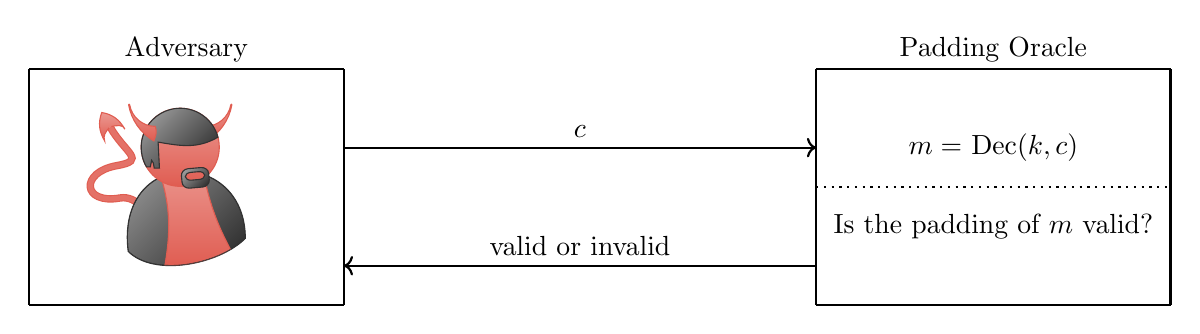
\begin{tikzpicture}
	\node[] (lblAdv) at (2,3.25) {Adversary};
	\draw[-,thick] (0,0)--(4,0);
	\draw[-,thick] (4,0)--(4,3);
	\draw[-,thick] (4,3)--(0,3);
	\draw[-,thick] (0,3)--(0,0);
	
	\node[devil, evil, minimum size=1.5cm] (Attacker) at (2,1.5) {};
	
	\node[] (lblCha) at (12.25,3.25) {Padding Oracle};
	\draw[-,thick] (10,0)--(14.5,0);
	\draw[-,thick] (14.5,0)--(14.5,3);
	\draw[-,thick] (14.5,3)--(10,3);
	\draw[-,thick] (10,3)--(10,0);
	
	\node[] (KeyGen) at (12.25,2) {$m =$ Dec$(k,c)$};
	\draw[-, thick, dotted] (10,1.5) -- (14.5,1.5);
	
	\draw[->, thick] (4,2) -- (10,2) node[midway, above] {$c$};
	\node[] (Mac) at (12.25,1) {Is the padding of $m$ valid?};

	\draw[<-,thick] (4,0.5) -- (10,0.5) node[midway, above] {valid or invalid};
\end{tikzpicture}
\end{document}
